\documentclass[11pt]{article}

\usepackage{kotex}
\usepackage{multirow}
\usepackage{latexsym}
\usepackage{color}
\usepackage{colortbl}
\usepackage[table]{xcolor}
\usepackage{sidecap}
\usepackage{graphicx}

\begin{document}
Hello world!

\begin{tabular}{r@{.}l}
3&14159 \\
16&2 \\
12345&689
\end{tabular}

\begin{tabular}{|c|c|c|} \hline
첫째 줄의 & 높이는 & 기본 높이 \\ \hline
이지만 & 둘째 줄의 & 높이는 \\ [1cm] \hline
1cm가 & 추가 & 되었다. \\  \hline
\end{tabular}

\begin{table}[t]
\caption{\texttt{tabular} 환경의 이용 보기\label{tab:t abular}}
\begin{center}
\begin{tabular}{l|cr}
성명 & 주소지 & 월수입 \\ \hline
김철수 & 서울 & 1,000,000 \\
이보라미 & 충청남도 & 60,000
\end{tabular}
\end{center}
\end{table}

\begin{table}
\caption{tabullar 환경으로 만든 보기--2\label{tab:tabular2}}
\begin{center}
\begin{tabular}{|r||r@{--}l|*{2}{c|}p{2in}|} \hline
\multicolumn{6}{|c|}{S 사의 주가} \\ \hline \hline
& \multicolumn{2}{|c|}{주가} & & & \\  \cline{2-3}
연도 & \multicolumn{1}{r@{\vline}}{최저} & 최고 & 거래량 & 액수 & \multicolumn{1}{c|}{특기 사항} \\ \hline
1972 & 97 & 172 & 111 & 12 & 상장 초기로서 특이 사항은 없으나 관심을 받았음 \\ \hline
83 & 130 & 200 & 1000 & 900 & 80+년대 초 \\  \hline
95 & \multicolumn{5}{|c|}{+이 자료는 가상임} \\ \hline
\end{tabular}
\end{center}
\end{table}

\begin{tabular}{l|l}
제 1 열 & 제 2 열 \\ \hline 
column 1 & column 2
\end{tabular}

{
\tabcolsep=0in
\begin{tabular}{l|l}
제 1 열 & 제 2 열 \\ \hline
column 1 & column 2
\end{tabular}}

\begin{tabbing}
김 철수 \= 통계학과 \\
이 미숙 \> 수학과 \\
야수 오모리 \> 경졔학과
\end{tabbing}

%\begin{tabbing}
%탭 설정만 \= \kill
%여기에 \> 탭 설정 \= 새 탭 설정 \+\+ \\
%세 번째 줄에 출력 \\
%\< \< 제 1 열 \> 제 2 열 \> 제 3 열 \\
%2열 \> 3 열 \- \\
%1 열 \\
%\pushtabs
%갑 \= 을 \\
%\> 병 \' 계는 오른쪽 끝 \\
%\poptabs
%가 \> 나 \> 다 \\
%\a={A} \> a'{A} \> a'{A}
%\end{tabbing}

\begin{tabular}{|l|l|} \hline
전체 행 & 개별 행 \\ \hline
\multirow{3}{*}{네 개의 행} & 1번 행 \\
& 2번 행 \\
& 3번 행 \\
& 4번 행 \\ \hline
합 & 네 개의 행 \\ \hline
\end{tabular}

\begin{tabular}{|l|l|} \hline
전체 행 & 개별 행 \\ \hline
\multirow{3}{*}[-8pt]{네 개의 행} & 1번 행 \\
& 2번 행 \\
& 3번 행 \\
& 4번 행 \\ \hline
합 & 네 개의 행 \\ \hline
\end{tabular}

%\setlongtable
%\begin{longtable}[c][l]{\hspace*{fill}}ll{\hspace*{\fill}ll}
%\caption{\texttt{longtable} 환경을 이용한 표 \label{tab:longtable}}
%\\ \hline \multicolumn{6}{c}{수학 모드의 부호들} \\ \hline
%출력 & 입력 & 출력 & 입력 & 출력 & 입력 \\ \hline \endfirsthead
%\caption[]{전 페이지에서 계속} \\ \hline
%출력 & 입력 & 출력 & 입력 & 출력 & 입력 \\ \hline \endhead
%\hline \multicolumn{6}{r}{다음 면에 계속} \\ \hline \endfoot
%\hline \multicolumn{6}{r}{표~\ref{tab:longtable}의 끝.}
%\\ \hline \endlastfoot
%\multicolumn{6}{c}{소문자} \\
%$\alpha$ & \verb+\alpha+ & $\beta$ & \verb+\beta+ & $\gamma$ & \verb+\grmma+ \\
%.
%.
%.
%\colorbox{mycyan}{$\lhd$}\myfootnote{\colorbox{mycyan}{\mbox{ }}표시된 부호는 \texttt{latexsym}  패키지를 사용할 때만 쓸 수 있음.}
%.
%.
%.
%\circledR & \verb+\circleR+ & \checkmark & \verb+\checkmark+ & \maltese & \verb+\maltese+ \\ \hline
%\end{longtable}

\begin{tabular}{|>{\columncolor[rgb]{0, .8, 0}[0pt]}l| >{\color{white}\columncolor[gray]{.2}[0pt]}l|}
Green & 바탕색 \\
By & \texttt{colortbl} 패키지 \\
And & 회색도 사용
\end{tabular}

\begin{tabular}{|>{\columncolor[rgb]{0, .8, 0}}l| >{\color{white}\columncolor[gray]{.2}}l|}
Green & 바탕색 \\
By & \texttt{colortbl} 패키지 \\
And & 회색도 사용
\end{tabular}

\begin{tabular}{|>{\columncolor[rgb]{0, .8, 0}}l|>{\color{white} \columncolor[gray]{.2}}l|}
Green & \cellcolor[gray]{.4}바탕색 \\
By & \texttt{colortbl} 패키지 \\
\rowcolor[rgb]{1,0,1} And & 회색도 사용
\end{tabular}

\setlength\arrayrulewidth{2pt}
\setlength\doublerulesep{2pt}
\arrayrulecolor{blue} \doublerulesepcolor{yellow}
\begin{tabular}{||l||c||} \hline \hline
줄을 & 굵기와 \\ \hline
폭을 & 일부러 \\ \hline
크게 & 하였음 \\ \hline\hline
\end{tabular}

{
\rowcolors[\hline]{1}{lime}{}
\begin{tabular}{ll}
\number \rownum & 가나 \\
\number \rownum & 가나 \\
3 & 가나 \\
4 & 가나 \\
\hiderowcolors
5 & 가나 \\
6 & 가나
\end{tabular}
}

\begin{SCfigure}
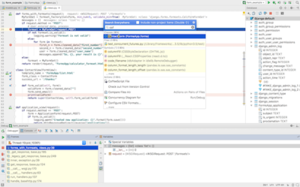
\includegraphics[width=0.6\textwidth]{../images/PyCharm_Screenshot.png}
\caption[\texttt{SCfigure} 환경의 그림]{\texttt{sidecap} 패키지의\texttt{SCfigure} 환경으로 만든 그림이다. 이 그림은 제목이 그림의 왼쪽 또는 오른쪽에 나타난다.\label{fig:scfig}}
\end{SCfigure}

\begin{figure}
\begin{center}

\includegraphics[width=3em]{../images/play.png}
\end{center}
\caption{그림 제목 들어가요.} \label{fig:play2}
\end{figure}





\end{document}